\documentclass[11pt,a4paper]{article}
\usepackage[margin=1in]{geometry}
\usepackage{booktabs}
\usepackage{longtable}
\usepackage{array}
\usepackage{hyperref}
\usepackage{graphicx}
\usepackage{tikz}
\usetikzlibrary{arrows.meta,positioning,shapes.geometric}

\title{Assignment 1: E-Purchase Business Process Modeling}
\author{CSE346/CSE345 Business Process Modeling}
\date{Spring 2026}

\begin{document}
\maketitle

\section{Scope and Tool Choice}
The modeled process is an Amazon/Souq-like e-purchase order-to-cash flow. It starts when a customer submits checkout details and ends when the order is delivered, archived, or rejected. The model follows the BPM lifecycle from the lectures: define objectives, model the as-is process, analyze issues, design the to-be process, then prepare implementation and monitoring.

\textbf{Primary online modeling tool:} \href{https://bpmn.io/}{bpmn.io} because Lecture 2 explicitly lists it as a BPMN tool and it supports BPMN 2.0 import/export in the browser. The generated BPMN XML files are:
\begin{itemize}
  \item \texttt{output/assignment1\_epurchase\_as\_is.bpmn}
  \item \texttt{output/assignment1\_epurchase\_to\_be.bpmn}
\end{itemize}
\textbf{Optional online validation/export tools:} Camunda Web Modeler for BPMN editing and diagrams.net for final image layout if a single-page polished figure is required. The report keeps BPMN 2.0 semantics as the source of truth.

\section{Lecture Concepts Applied}
The report uses these concepts from the LECS folder:
\begin{itemize}
  \item BPM models make invisible work visible and support analysis before automation.
  \item BPMN Business Process Diagrams consist of flow objects, connections, swimlanes, and artifacts.
  \item XOR gateways model exclusive decisions; AND gateways model parallel work and synchronization.
  \item Pools and lanes represent participants, roles, departments, systems, and handoffs.
  \item Intermediate timer/message events represent events that occur during process execution.
  \item Process analysis evaluates cycle time, capacity, cost, quality, risk, and customer interfaces.
  \item Redesign patterns include eliminating waste, introducing parallelism, improving communication, using IT-driven improvements, and appointing process/case managers.
\end{itemize}

\section{As-Is BPMN Model}
\subsection{Participants and Data}
\begin{longtable}{p{0.25\linewidth}p{0.65\linewidth}}
\toprule
Participant or lane & Responsibility \\
\midrule
Customer & Places order, provides address, receives invoice and delivery, may complain about delay. \\
Marketplace system & Captures order, checks stock, validates address, emits invoice, archives order. \\
Payment service & Authorizes payment and confirms payment status. \\
Warehouse & Reserves item, picks, packs, and prepares shipment. \\
Courier & Ships product and reports delivery status. \\
Customer support & Registers complaints and escalates delayed shipments. \\
\bottomrule
\end{longtable}

\subsection{As-Is Control Flow}
\begin{center}
\resizebox{\linewidth}{!}{%
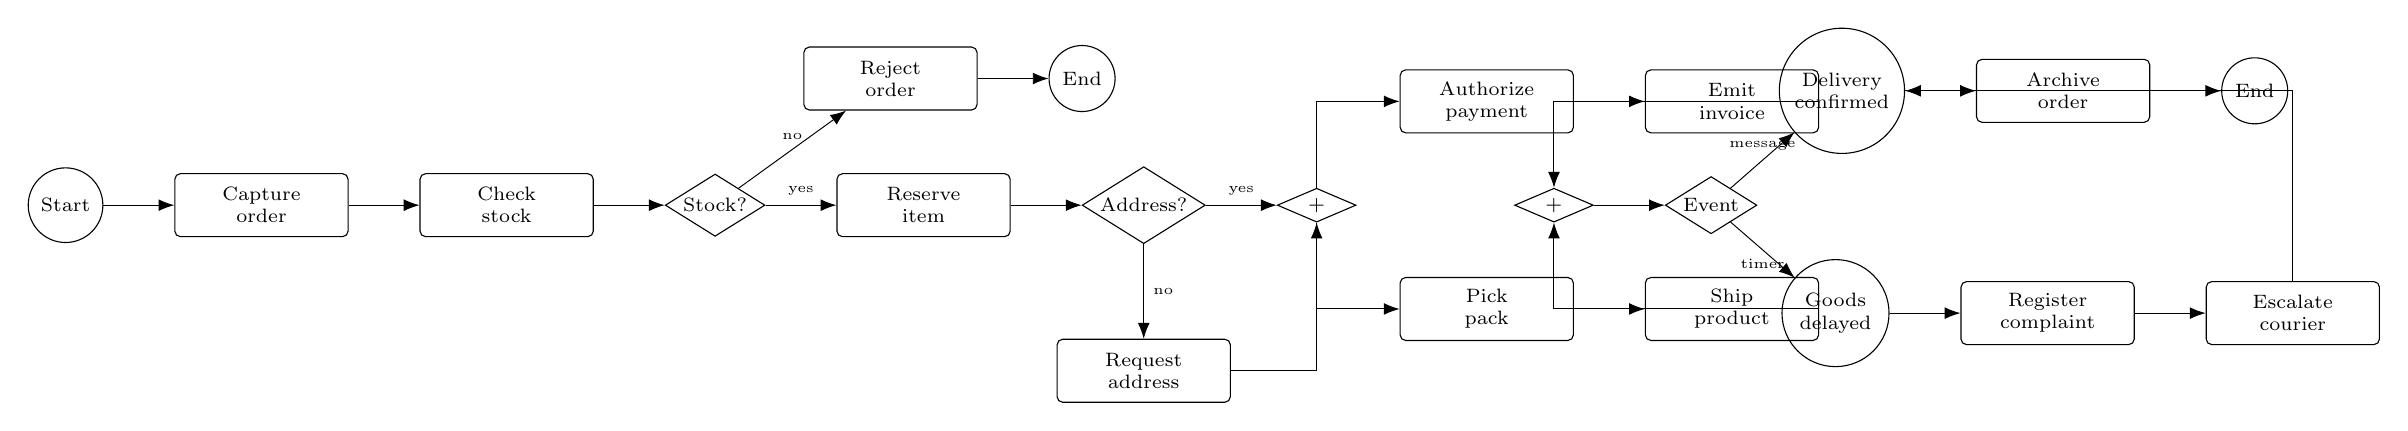
\begin{tikzpicture}[
  node distance=7mm and 9mm,
  task/.style={draw, rounded corners=2pt, minimum width=22mm, minimum height=8mm, align=center, font=\scriptsize},
  gateway/.style={draw, diamond, aspect=1.6, minimum width=10mm, align=center, font=\scriptsize, inner sep=1pt},
  event/.style={draw, circle, minimum size=8mm, align=center, font=\scriptsize},
  flow/.style={-{Latex[length=2mm]}, line width=0.35pt}
]
\node[event] (start) {Start};
\node[task, right=of start] (capture) {Capture\\order};
\node[task, right=of capture] (stock) {Check\\stock};
\node[gateway, right=of stock] (gstock) {Stock?};
\node[task, above right=10mm and 8mm of gstock] (reject) {Reject\\order};
\node[event, right=of reject] (endrej) {End};
\node[task, right=of gstock] (reserve) {Reserve\\item};
\node[gateway, right=of reserve] (gaddr) {Address?};
\node[task, below=12mm of gaddr] (reqaddr) {Request\\address};
\node[gateway, right=of gaddr] (fork) {+};
\node[task, above right=8mm and 8mm of fork] (pay) {Authorize\\payment};
\node[task, right=of pay] (invoice) {Emit\\invoice};
\node[task, below right=8mm and 8mm of fork] (pick) {Pick\\pack};
\node[task, right=of pick] (ship) {Ship\\product};
\node[gateway, right=20mm of fork] (join) {+};
\node[gateway, right=of join] (evgw) {Event};
\node[event, above right=7mm and 8mm of evgw] (delivered) {Delivery\\confirmed};
\node[event, below right=7mm and 8mm of evgw] (late) {Goods\\delayed};
\node[task, right=of late] (complaint) {Register\\complaint};
\node[task, right=of complaint] (escalate) {Escalate\\courier};
\node[task, right=of delivered] (archive) {Archive\\order};
\node[event, right=of archive] (end) {End};
\draw[flow] (start) -- (capture);
\draw[flow] (capture) -- (stock);
\draw[flow] (stock) -- (gstock);
\draw[flow] (gstock) -- node[above,font=\tiny]{no} (reject);
\draw[flow] (reject) -- (endrej);
\draw[flow] (gstock) -- node[above,font=\tiny]{yes} (reserve);
\draw[flow] (reserve) -- (gaddr);
\draw[flow] (gaddr) -- node[above,font=\tiny]{yes} (fork);
\draw[flow] (gaddr) -- node[right,font=\tiny]{no} (reqaddr);
\draw[flow] (reqaddr.east) -| (fork.south);
\draw[flow] (fork) |- (pay);
\draw[flow] (pay) -- (invoice);
\draw[flow] (invoice.east) -| (join.north);
\draw[flow] (fork) |- (pick);
\draw[flow] (pick) -- (ship);
\draw[flow] (ship.east) -| (join.south);
\draw[flow] (join) -- (evgw);
\draw[flow] (evgw) -- node[above,font=\tiny]{message} (delivered);
\draw[flow] (evgw) -- node[below,font=\tiny]{timer} (late);
\draw[flow] (late) -- (complaint);
\draw[flow] (complaint) -- (escalate);
\draw[flow] (escalate.north) |- (delivered.east);
\draw[flow] (delivered) -- (archive);
\draw[flow] (archive) -- (end);
\end{tikzpicture}
}
\end{center}

The goods-delay requirement is modeled by an intermediate timer event after shipment. If delivery confirmation is not received within the SLA, the timer branch opens a complaint and escalates the courier. This follows the lecture definition of an intermediate timer event: it is enabled during the process and fires after a time interval elapses.

\section{As-Is Analysis}
\begin{longtable}{p{0.07\linewidth}p{0.19\linewidth}p{0.30\linewidth}p{0.16\linewidth}p{0.18\linewidth}}
\toprule
No. & Issue & Consequence & Type & Proposed fix \\
\midrule
1 & Late complaint is reactive & Customer discovers delay before the company does; poor external quality. & Process / customer interface & Add proactive shipment tracking and automatic SLA monitoring. \\
2 & Address collection may happen after stock reservation & Reserved stock can wait while customer data is corrected. & Data / process & Validate address at checkout before reservation. \\
3 & Payment and fulfillment handoffs are loosely synchronized & Manual checks can delay either invoice or shipment. & IT / organization & Run payment authorization and stock checks in parallel. \\
4 & Complaint path is separate from normal case ownership & Support may not have full order context. & Organization & Assign a case owner and attach complaint to the same order case. \\
5 & Archive occurs only at the end & Operational data may be unavailable for monitoring until closure. & IT & Record status events throughout the process. \\
\bottomrule
\end{longtable}

The main performance risks are waiting time and handoff delay. The lectures define cycle time as the time from process start to end; in this process, cycle time is affected by address correction, payment confirmation, shipment waiting time, and complaint escalation. Several steps are business-value adding, such as payment control and archiving, but waiting for missing data and discovering delays late are waste.

\section{To-Be BPMN Model}
\begin{center}
\resizebox{\linewidth}{!}{%
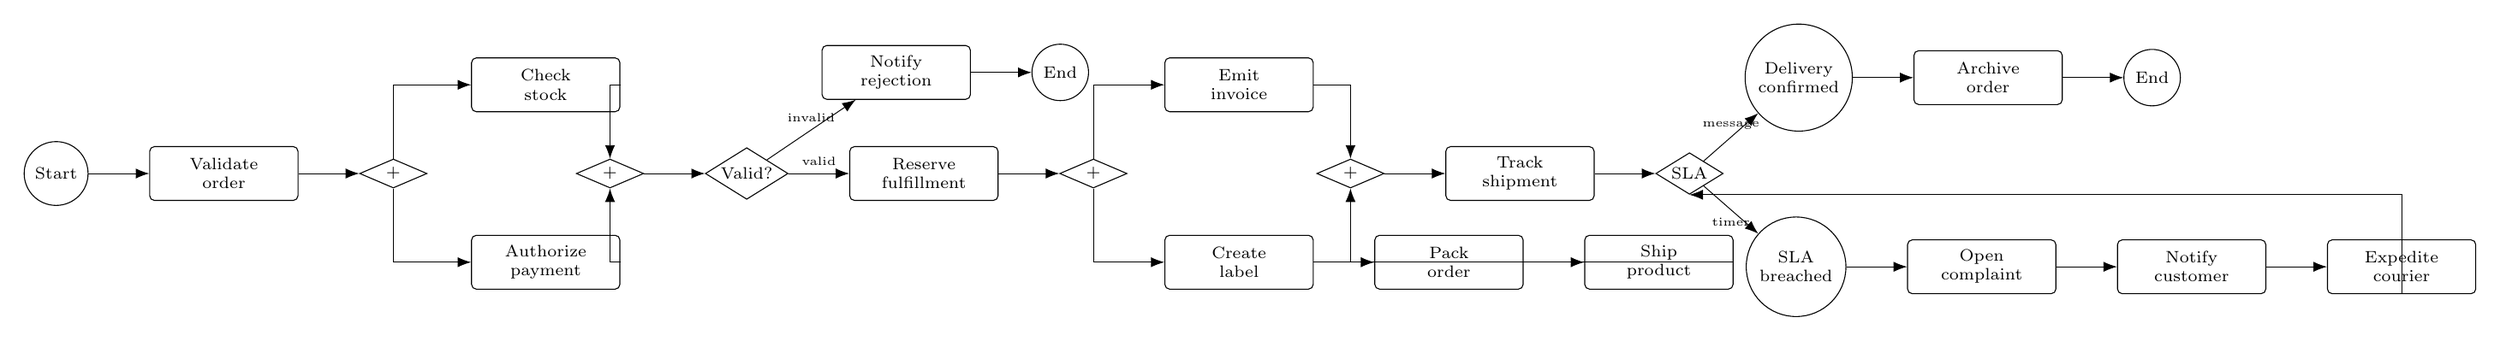
\begin{tikzpicture}[
  node distance=7mm and 9mm,
  task/.style={draw, rounded corners=2pt, minimum width=22mm, minimum height=8mm, align=center, font=\scriptsize},
  gateway/.style={draw, diamond, aspect=1.6, minimum width=10mm, align=center, font=\scriptsize, inner sep=1pt},
  event/.style={draw, circle, minimum size=8mm, align=center, font=\scriptsize},
  flow/.style={-{Latex[length=2mm]}, line width=0.35pt}
]
\node[event] (start) {Start};
\node[task, right=of start] (validate) {Validate\\order};
\node[gateway, right=of validate] (checks) {+};
\node[task, above right=8mm and 9mm of checks] (stock) {Check\\stock};
\node[task, below right=8mm and 9mm of checks] (pay) {Authorize\\payment};
\node[gateway, right=22mm of checks] (join1) {+};
\node[gateway, right=of join1] (valid) {Valid?};
\node[task, above right=9mm and 8mm of valid] (reject) {Notify\\rejection};
\node[event, right=of reject] (endrej) {End};
\node[task, right=of valid] (reserve) {Reserve\\fulfillment};
\node[gateway, right=of reserve] (fork) {+};
\node[task, above right=8mm and 8mm of fork] (invoice) {Emit\\invoice};
\node[task, below right=8mm and 8mm of fork] (label) {Create\\label};
\node[task, right=of label] (pack) {Pack\\order};
\node[task, right=of pack] (ship) {Ship\\product};
\node[gateway, right=28mm of fork] (join2) {+};
\node[task, right=of join2] (track) {Track\\shipment};
\node[gateway, right=of track] (sla) {SLA};
\node[event, above right=7mm and 8mm of sla] (delivered) {Delivery\\confirmed};
\node[event, below right=7mm and 8mm of sla] (late) {SLA\\breached};
\node[task, right=of late] (open) {Open\\complaint};
\node[task, right=of open] (notify) {Notify\\customer};
\node[task, right=of notify] (expedite) {Expedite\\courier};
\node[task, right=of delivered] (archive) {Archive\\order};
\node[event, right=of archive] (end) {End};
\draw[flow] (start) -- (validate);
\draw[flow] (validate) -- (checks);
\draw[flow] (checks) |- (stock);
\draw[flow] (checks) |- (pay);
\draw[flow] (stock.east) -| (join1.north);
\draw[flow] (pay.east) -| (join1.south);
\draw[flow] (join1) -- (valid);
\draw[flow] (valid) -- node[above,font=\tiny]{invalid} (reject);
\draw[flow] (reject) -- (endrej);
\draw[flow] (valid) -- node[above,font=\tiny]{valid} (reserve);
\draw[flow] (reserve) -- (fork);
\draw[flow] (fork) |- (invoice);
\draw[flow] (fork) |- (label);
\draw[flow] (label) -- (pack);
\draw[flow] (pack) -- (ship);
\draw[flow] (invoice.east) -| (join2.north);
\draw[flow] (ship.east) -| (join2.south);
\draw[flow] (join2) -- (track);
\draw[flow] (track) -- (sla);
\draw[flow] (sla) -- node[above,font=\tiny]{message} (delivered);
\draw[flow] (sla) -- node[below,font=\tiny]{timer} (late);
\draw[flow] (late) -- (open);
\draw[flow] (open) -- (notify);
\draw[flow] (notify) -- (expedite);
\draw[flow] (expedite.south) |- (sla.south);
\draw[flow] (delivered) -- (archive);
\draw[flow] (archive) -- (end);
\end{tikzpicture}
}
\end{center}

\section{Enhancements and Comparative Analysis}
\begin{longtable}{p{0.24\linewidth}p{0.31\linewidth}p{0.31\linewidth}}
\toprule
Area & As-is & To-be improvement \\
\midrule
Checkout data & Address may be requested after stock reservation. & Validate address, stock, and payment early. \\
Cycle time & Sequential checking increases waiting. & Stock and payment checks run in parallel, following the lecture redesign pattern of introducing parallelism. \\
Delay handling & Complaint starts only after a late delivery event. & SLA timer creates a proactive complaint and customer notification. \\
Quality & Customer may have to ask for status. & Tracking status is recorded and communicated automatically. \\
Cost and rework & Support may manually reconstruct order context. & Complaint is attached to the same order case with a case owner. \\
Flexibility & Same path for all orders after basic stock check. & Exceptions are explicit: invalid order, SLA breach, courier escalation, and final delivery. \\
\bottomrule
\end{longtable}

Expected outcomes are shorter average cycle time, fewer avoidable waiting periods, better customer-facing quality, and improved monitoring. There is a trade-off from the process analysis lecture: the to-be model has more IT coordination and status events, but it reduces waiting, communication errors, and complaint handling cost.

\section{Case Coverage}
\begin{itemize}
  \item Normal successful order: checkout, stock/payment validation, fulfillment, delivery, archive.
  \item Out-of-stock or invalid payment: notify rejection and end rejected.
  \item Missing or invalid address: caught at validation before stock is reserved.
  \item Shipment delivered on time: delivery message event continues to archive.
  \item Goods delayed: intermediate timer event opens complaint, notifies customer, escalates courier, and loops back to wait for delivery status.
  \item Operational audit: archive order and status events support monitoring and future process mining.
\end{itemize}

\section{Submission Checklist}
The zipped submission should include this report PDF, the two BPMN XML files, and exported images from bpmn.io or Camunda if required by the instructor. The BPMN files were generated by \texttt{tools/generate\_assignment1\_bpmn.py}, then can be imported into the selected online BPMN tool.

\end{document}
